\section{Experiments}
\label{exp}
In Section \ref{exp}, we explain the experiment process in detail, including datasets, experimental setup, implementation details and evaluation results.

\subsection{Dataset}
\label{dataset}
Experiments are done on two datasets: FewRel dataset \cite{han-etal-2018-fewrel} and our proposed TinyRel-CM dataset.
~\\
~\\
\textbf{FewRel Dataset} FewRel dataset \cite{han-etal-2018-fewrel} is a few-shot relation classification dataset constructed through distant supervision and human annotation. It consists of 100 relation classes with 700 instances per class. The relation classes are split into subsets of size 64, 16 and 20 for training, validation and testing, respectively.
The average length of a sentence in FewRel dataset is 24.99, and there are 124,577 unique tokens in total. By the time of writing, FewRel is the only few-shot relation classification dataset available.
~\\
~\\
\textbf{TinyRel-CM Dataset} TinyRel-CM dataset is our proposed Chinese few-shot relation classification dataset in health domain with limited training data. The TinyRel-CM dataset is constructed through the following steps: (1) Crawl data from Chinese health-related websites \footnote{\url{www.9939.com}, \url{www.39.net}, and \url{www.xywy.com}} to form a large corpus and an entity dictionary. (2) Automatically align entities in the corpus with the entity dictionary, forming a large candidate-sentence set. (3) 5 Chinese medical students manually filter out the unqualified candidate sentences and tag qualified ones with corresponding class labels. An instance is added to the dataset only if 3 or more annotators make consistent decisions. This process costs 4 days.

The TinyRel-CM Dataset consists of 27 relation classes with 50 instances per class. The 27 relation classes cover binary relations among 4 entity types, and are grouped into 6 categories according to the entity types, forming 6 tasks with one group being the test set and other 5 groups serving as training set (see Table \ref{Egroup}). An example instance in the TinyRel-CM dataset is shown in Tabel \ref{FRMexample}. The average length of a sentence in TinyRel-CM dataset is 67.31, and there are 2,197 unique characters in total. Comparison of TinyRel-CM dataset and FewRel dataset is shown in Table \ref{Datasetcompare}.

\begin{table}[ht]
\centering
\small
\begin{tabu}{|c|[0.5pt]l|}
\hline
\textbf{Group} & \textbf{Classes} \\ \tabucline[0.5pt]{-}
D-D & complication, cause, is, include, NA \\ \hline
D-S & have, NA\\ \hline
D-F & positive, negative, forbid, prevent, cause, NA\\ \hline
D-U & positive, negative, prevent, lack, cause, NA\\ \hline
F-U & contain, NA\\ \hline
S-F & forbid, cause, positive, negative, prevent, NA\\ \hline
\end{tabu}
\caption{Entity groups in TinyRel-CM dataset. D,S,F, and U stand for Disease, Symptom, Food, and nUtrient, respectively.}
\label{Egroup}
\end{table}

\begin{table}[ht]
\centering
\small
\begin{tabular}{|l|p{170pt}|}
\hline
\textbf{Group} & D-D \\ \hline %\tabucline[1pt]{-}
\textbf{Class} & complication \\ \hline
\textbf{Explanation} & Entity 2 is a complication of entity 1. \\ \hline
\multirow{2}{*}{\textbf{Example}} & [子宫肌瘤]$_{entity1}$出现了[慢性盆腔炎]$_{entity2}$并发症,导致月经量过多。 \\
& \textcolor[rgb]{0.45,0.45,0.45}{Once [Hysteromyoma]$_{entity1}$ is complicated with [chronic pelvic inflammation]$_{entity2}$, menstruation increase.}  \\ \hline
\end{tabular}
\caption{An example instance in the TinyRel-CM dataset.}
\label{FRMexample}
\end{table}


\begin{table}[ht]
\centering
\small
\begin{tabular}{|l|r|r|r|}
\hline
\textbf{Dataset} & \textbf{\#cls.} & \textbf{\#inst./cls.} & \textbf{\#inst.} \\ \hline
FewRel & 100 & 700 & 70,000 \\ \hline
TinyRel-CM & 27 & 50 & 1,350 \\ \hline
\end{tabular}
\caption{Comparison of TinyRel-CM dataset to FewRel dataset.}
\label{Datasetcompare}
\end{table}


The TinyRel-CM dataset is harder than FewRel dataset for two reasons. On one hand, the training data size is small (as is shown in Table \ref{Datasetcompare}). On the other hand, the relation classes in a given test set are relative to each other since they share common entity types (because the classes are from the same entity group). In other datasets, the entity types are distinct in most situations, which may serve as extra information. %Figure xx shows example instances from previous datasets and the HEALTHXX dataset. For previous datasets, the instances within the same category is likely to be quite similar while instances from different categories distinct from one to another. While in HEALTHXX datasets, the format of instances within one category varies from one to another, which makes the task harder.

%
%\begin{table*}[hbt]
%\centering
%\tiny
%\begin{tabular}{|l|c|p{8pt}<{\centering}p{8pt}<{\centering}p{8pt}<{\centering}p{8pt}<{\centering}p{8pt}<{\centering}|p{8pt}<{\centering}p{8pt}<{\centering}p{8pt}<{\centering}p{8pt}<{\centering}p{8pt}<{\centering}|p{8pt}<{\centering}p{8pt}<{\centering}p{8pt}<{\centering}p{8pt}<{\centering}p{8pt}<{\centering}|p{8pt}<{\centering}p{8pt}<{\centering}p{8pt}<{\centering}p{8pt}<{\centering}p{8pt}<{\centering}|}
%\hline
%\multirow{3}{*}{\textbf{Method}} & \textbf{+} & \multicolumn{5}{c|}{\emph{- -}} &\multicolumn{5}{c|}{\emph{MME}} & \multicolumn{5}{c|}{\emph{Data}} & \multicolumn{5}{c|}{\emph{MME\&Data}} \\ \cline{2-22}
%& \multirow{2}{*}{\textbf{(N,K)}} & \multicolumn{20}{c|}{\textbf{Shrink origin training set size to }} \\ \cline{3-22}
%& &L0 &L1 &L2 &L3 & L4 & L0&  L1 &L2 &L3 & L4 &L0 & L1 &L2 &L3 & L4 & L0 & L1 &L2 &L3 & L4 \\ \hline
%\multirow{4}{*}{MetaN} & (~~5,1) &&&&& &&&&& &&&&& &&&&&\\
%& (~~5,5) &&&&& &&&&& &&&&& &&&&& \\
%& (10,1) &&&&& &&&&& &&&&& &&&&&\\
%& (10,5) &&&&& &&&&& &&&&& &&&&& \\ \hline
%\multirow{4}{*}{GNN} & (~~5,1) &61.87&53.95 &42.59 & 40.88&24.51   &63.20&55.81&46.85&40.61&23.09   &56.71&\textbf{58.40}&50.99&\textbf{51.92}&39.97    &\textbf{63.70} &56.83&\textbf{52.64}&48.26&\textbf{45.38}\\
%& (~~5,5)& 73.92&68.21 &55.16 & 52.24&28.94   &76.62&68.92&61.19&50.56&27.63    &70.76 &\textbf{71.96}&64.87&\textbf{66.17}&48.30     &\textbf{77.13} &71.42&\textbf{66.47}&60.94&\textbf{54.54}\\
%& (10,1) &53.32&38.57 &30.38 &28.08&18.91   &\textbf{54.87}&37.06&35.59&29.98&15.36    &54.81 &\textbf{43.99}&\textbf{37.64}&33.85&\textbf{30.32}     &54.23&42.53&36.98&\textbf{36.32}&29.36\\
%& (10,5) &65.64&52.07 &39.78 & 38.03&24.25   &67.15&51.41&47.91&41.05&20.03    &66.76 &\textbf{57.97}&50.33&47.74&\textbf{40.23}      &\textbf{67.80}&56.60&\textbf{50.85}&\textbf{49.73}&40.18\\ \hline
%
%\multirow{4}{*}{SNAIL} & (~~5,1) &29.85&\textbf{44.67}&33.36&33.64&20.85   &\textbf{48.25}&36.08&36.21&29.32&27.72     &30.82&42.40&35.38&35.32&28.26    &43.10&42.76&\textbf{39.70}&\textbf{39.08}&\textbf{34.32} \\
%& (~~5,5)&55.39 &53.62&46.66&38.41&28.81    &55.76&\textbf{61.36}&55.91&39.46&26.85     &\textbf{63.38}&57.74&48.68&43.70&20.02     &56.04&51.32&\textbf{56.44}&\textbf{44.04}&\textbf{38.28} \\
%& (10,1) &35.16&22.64&25.33&19.60&11.67    &35.43&\textbf{27.37}&24.07&24.65&15.72     &38.49&26.34&\textbf{27.19}&\textbf{28.00}&19.85     &\textbf{43.51}&26.52&25.85&27.77&\textbf{29.25}\\
%& (10,5) &47.73&36.40&\textbf{40.94}&\textbf{27.92}&13.08    &48.65&42.17&36.86&26.43&15.01     &\textbf{54.06}&37.36&31.92&23.51&25.57     &52.14&\textbf{42.18}&33.38&27.30&\textbf{26.34}\\ \hline
%
%\multirow{4}{*}{Proto} & (~~5,1) &71.50&67.94 &61.37 & 58.20&35.68   &71.44&66.98 &65.04 &59.25&40.04   &71.78&69.47&64.80&\textbf{64.48}&\textbf{61.19}  &\textbf{72.03}&\textbf{71.06}&\textbf{68.85}&63.83&59.85 \\
%& (~~5,5) &82.72&79.49 &74.05 & 72.60&49.82  &83.01&79.82 &79.04 &74.22&56.24   &84.09&81.60&78.28&\textbf{77.96}&\textbf{74.62}   &\textbf{84.29}&\textbf{82.66}&\textbf{81.20}&77.43&73.78 \\
%& (10,1) &57.53&52.63 &45.16 & 44.23&22.30    &57.70&52.44 &50.03 &44.87&25.72   &58.58&55.77&49.91&\textbf{50.25}&\textbf{46.45}   &\textbf{58.80}&\textbf{56.38}&\textbf{54.05}&50.01&45.01\\
%& (10,5) &70.95&65.76 &59.21 & 58.23&34.34    &71.13&66.18 &65.42 &59.85&40.11   &72.46&68.96&64.05&\textbf{64.82}&\textbf{60.58}   &\textbf{72.70}&\textbf{70.04}&\textbf{68.22}&64.23&60.02\\ \hline
%
%
%\multirow{4}{*}{HATT} & (~~5,1) &&&&& &&&&& &&&&& &&&&&\\
%& (~~5,5) &&&&& &&&&& &&&&& &&&&&\\
%& (10,1) &&&&& &&&&& &&&&& &&&&&\\
%& (10,5) &&&&& &&&&& &&&&& &&&&&\\ \hline
%
%\multirow{4}{*}{MLMAN} & (~~5,1) &76.82\footnotemark[1] &69.98 &69.69 &64.63 &57.70    &76.95& 72.92& 70.58&65.24 &59.15    &77.06&\textbf{72.97} & 68.36& 66.97&\textbf{67.22}   &\textbf{77.35}&72.89 &\textbf{72.45} & \textbf{68.84} &66.49\\
%& (~~5,5) &87.46\footnotemark[1]&84.40 &83.64 & 79.71&72.62   &87.63& 86.26& 83.71&80.20 & 74.71    &87.80 &86.41 &83.98 & 83.05&81.39   &\textbf{88.31}& \textbf{86.49} & \textbf{85.92}& \textbf{84.21} &\textbf{81.87} \\
%& (10,1) &64.15\footnotemark[1]&57.96 &56.48 & 50.60&43.61   &65.70&\textbf{61.55} & 58.49&51.42 & 44.45   &65.55&61.32 & 55.82& 53.45&\textbf{53.74}   &\textbf{66.17}&61.16 &\textbf{60.00} & \textbf{56.02} &53.19 \\
%& (10,5) &78.55\footnotemark[1]&74.51 &72.42 & 67.52&58.62    &78.94& 76.45& 73.64&67.93 & 61.20   &\textbf{79.68}&76.27 & 72.48&71.05 &70.26   &79.53&\textbf{76.64} & \textbf{76.00}& \textbf{73.55} &\textbf{70.31}\\ \hline
%
%
%\multirow{4}{*}{BP} & (~~5,1) &85.38&79.89 &78.59 &71.89 &62.09     &86.06&77.70&77.48&76.74&64.82   &84.90&80.22&78.26&77.24&71.74  &\textbf{86.28}&\textbf{80.46}&\textbf{81.78}&\textbf{80.68}&\textbf{73.42}\\
%& (~~5,5) &87.51&83.49 &82.98 & 79.38&71.53  &87.65&82.12&82.80&83.34&74.41   &88.06&82.98&84.15&82.42&76.89   &\textbf{88.83}&\textbf{84.57}&\textbf{84.32}&\textbf{85.58}&\textbf{79.46}\\
%& (10,1) &\textbf{75.62}&69.13 &68.33 &63.08 &56.53  &75.22&68.92&68.09&67.06&54.95   &75.15&\textbf{70.21}&67.62&66.44&61.19     &75.55&68.60&\textbf{71.26}&\textbf{71.06}&\textbf{62.58}\\
%& (10,5) &79.23&72.99 &72.71 &69.53&63.31  &79.31&72.57&\textbf{73.75}&73.17&63.69   &79.29&72.18&72.67&72.30&65.20   &\textbf{79.34}&\textbf{74.04}&72.80&\textbf{75.72}&\textbf{67.20}\\
%
%\hline
%\end{tabular}
%\caption{Classification accuracy(\%) on FewRel validation set under N way K shot test configuration. MetaN, Proto, HATT and BP stand for Meta Networks, Prototypical Networks, Proto-HATT and Bert-Pair respectively.
%Meta Networks, SNAIL, GNN, SNAIL and Proto-HATT require the number of classes while training and testing to be equal. So a model is trained with N way tasks to perform N way tests. For SNAIL, the number of instances per relation while training and testing need to be equal. So a model is trained with K shot tasks to perform K shot test tasks.}
%\label{FewRelval}
%\end{table*}



\subsection{Experimental Setup}
%Totally three experiments are conducted to show the effectiveness of the proposed MSI framework and data augmentation method.
On the FewRel dataset, following \cite{han-etal-2018-fewrel,ye-ling-2019-multi}, we train the model with 20 way 10 shot training tasks and test with 4 configurations: 5 way 1 shot, 5 way 5 shot, 10 way 1 shot and 10 way 5 shot.

On the TinyRel-CM Dataset, for each group of relation classes, we adopt $x$ way 5 shot, $x$ way 10 shot and $x$ way 15 shot test configurations, where $x$ is the number of classes within the group. During training episodes, we conduct 5 way 15 shot training tasks. Thus totally 6 experiments are done.

For ablation test, in addition to applying the whole MESDA framework, we also apply the two proposed methods, support classifier and data augmentation, individually on baseline models.

Additionally, on the FewRel dataset, we reform the training set by shrinking the number of relation classes and instances per class to different extent. For each shrunken training set, we conduct different training task settings (shown in Table \ref{trainingsetting}) and test with 4 configurations: 5 way 1 shot, 5 way 5 shot, 10 way 1 shot and 10 way 5 shot over all shrunken training set. We do not further shrink the training data in TinyRel-CM dataset because its training data size is already small.

\begin{table}[ht]
\centering
\small
\begin{tabular}{|c|c|c|l|}
\hline
\textbf{\% of full training set} & \textbf{\#cls.} & \textbf{\#inst./cls.} & \textbf{Training task} \\ \hline
%100.00 & 64 & 700 & 20 way 10 shot  \\ \hline
7.00 & 30 & 100 & ~5 ~way 15 shot  \\ \hline
2.23 & 20 & 50 & ~5 ~way 15 shot \\ \hline
1.00 & 15 & 30 & ~5 ~way 10 shot \\ \hline
0.22 & 10 & 10 & ~5 ~way ~5~ shot \\ \hline
\end{tabular}
\caption{Training task settings over shrunken training set.}
\label{trainingsetting}
\end{table}

For all experiments, we randomly pick 2000 tasks and calculate the average accuracy in testing.

%All test results are represented as mean and standard deviation values of 10 repetitions.
%\subsection{Baselines}
%Prototypical networks(CNN)(PCNN) core
%MLMAN
%\textbf{Prototypical Network} Prototypical network is first proposed by \cite{proto}. The model assumes that there exists a prototype for each class that can represent the meaning of the class. The prototype vector of each class is calculated by averaging the representation vectors of the support instances in this class. When classifying a query instance into certain class, the model chooses the relation with the nearest prototype vector to be the prediction. \cite{han-etal-2018-fewrel} combined prototypical network with CNN/PCNN core to handle few-shot relation classification tasks.
%~\\
%~\\
%\textbf{MLMAN} Multi-Level Matching and Aggregation Network(MLMAN)\cite{ye-ling-2019-multi} also assumes that prototypes exist. The MLMAN model encodes both each query sentence and each support sentence in an interactive way by adding mutual information at both local and instance levels. The prototype of each relation class is calculated by attentively aggregating the support vectors of this relation. The weight of each support sentence is calculated regarding to the query instances.

\subsection{Implementation Details}
%\KZ{Reduce this section}
%\begin{table}[htbp]
%\centering
%\small
%\begin{tabular}{|c|c|c|}
%\hline
%\textbf{Component} & \textbf{Parameter} & \textbf{Value} \\ \hline
%ENG word embed & dimension & 50 \\ \hline
%CHN char embed & dimension & 100 \\ \hline
%\multirow{2}{*}{position embed} & max relative distance & $\pm80$ \\ \cline{2-3}
%& dimension & 5 \\ \hline
%\multirow{2}{*}{CNN} & window size & 3 \\ \cline{2-3}
%& filter number & 200 \\ \hline
%dropout & dropout rate & 0.2 \\ \hline
%unidirectional LSTM & hidden size & 100 \\ \hline
%\multirow{3}{*}{fast learner} & strategy & SGD \\ \cline{2-3}
%& initial learning rate & 0.1 \\ \cline{2-3}
%& learning rate decay & False \\ \hline
%\multirow{3}{*}{slow learner} & strategy & SGD \\ \cline{2-3}
%& initial learning rate & 0.1 \\ \cline{2-3}
%& learning rate decay & True \\ \hline
%\end{tabular}
%\caption{Hyper-parameters chosen in experiments.}
%\label{hyper}
%\end{table}

During implementation, we apply our framework and data augmentation method to the following baselines:
%(1) meta network \cite{metanet},
%(1)
GNN \cite{gnn},
%(2)
SNAIL \cite{snail},
%(3)
prototypical networks \cite{proto},
%(4)
proto-HATT \cite{hatt},
%(5)
MLMAN \cite{ye-ling-2019-multi}, and
%(6)
Bert-Pair \cite{gao-etal-2019-fewrel}.
%(1) Meta Network \cite{metanet}, which implements a high level meta learner based on the conventional learner.
%(2) GNN \cite{gnn}, which regards support and query instances as nodes in a graph.
%(3) SNAIL \cite{snail}, which aggregates attention into meta learner.
%(4) Prototypical Networks \cite{proto}, which assumes that each relation has a prototype and classifies a query instance into the relation of the closest prototype.
%(5) Proto-HATT \cite{hatt}, which reinforces the prototypical networks with hybrid attention mechanism.
%(6) MLMAN \cite{ye-ling-2019-multi}, which improves prototypical networks by aggregating local and instance-level attentions.
%(7) Bert-Pair \cite{gao-etal-2019-fewrel}, which adopts BERT \cite{devlin2018bert} to compute the possibility that a support instance and a query instance belong to the same class.

%For baselines (1) to (6), we keep the context encoder and class matching function and add supplementary classifier that receives each support instance as input. For baseline (7), due to the different structure, the supplementary classifier receives the concatenation of two support instances as input and outputs the probability of the two instances belonging to the same class.
%Codes for baseline (1) are provided by \cite{han-etal-2018-fewrel}.
Codes for GNN, SNAIL and Bert-Pair are provided by Gao et al. \shortcite{gao-etal-2019-fewrel}. Prototypical networks is our own implementation. Codes for proto-HATT and MLMAN are provided in the original paper.
%Codes for baselines (1), (2), and (6) are provided by \cite{gao-etal-2019-fewrel}. Baseline (3) uses our own implementation. For baselines (4), and (5) we use the codes provided in the original paper.

Due to the special architecture, the support classifier applied on Bert-Pair receives support instance pairs as input and computes the probability of the pairs belonging to the same class, different from other baselines.
%we choose MLMAN\cite{ye-ling-2019-multi} as the core model to provide the context encoder and class matching function. The context encoder consists of a CNN for encoding and a unidirectional LSTM for adding local and instance-level attention.

GNN, SNAIL, and proto-HATT require the number of classes while training and testing to be equal. So a model is trained with $N$ way tasks to perform $N$ way tests. In SNAIL and proto-HATT, the number of instances per class while training and testing need to be equal. So a model is trained with $K$ shot tasks to perform $K$ shot test tasks.

We keep the original hyper parameters for each baseline, and set the learning rate of the fast learner $0.1$. The supplementary data for TinyRel-CM dataset are from Chinese Literature NER RE dataset \cite{dnerre} (13,297 instances covering 10 classes) and Chinese Information Extraction dataset \cite{augdata} (1,100 instances covering 12 classes). Supplementary data for FewRel dataset is from NYT-10 dataset \cite{NYTdataset} which contains 143,391 instances over 57 classes (class \emph{NA} is removed during augmentation).

\begin{table}[ht]
\centering
\scriptsize
\begin{tabular}{|l|c|p{25pt}<{\centering}|p{25pt}<{\centering}|p{25pt}<{\centering}|p{25pt}<{\centering}|}
\hline
%\multirow{2}{*}{\textbf{Method}} & \textbf{+} & \multirow{2}{*}{\emph{-}} & \multirow{2}{*}{\emph{MME}} & \multirow{2}{*}{\emph{data}} &\multirow{2}{*}{\emph{MME\&data}} \\ \cline{2-6}
%& \textbf{(N,K)} & &&&\\ \hline
\textbf{Method} & \textbf{(N,K)}& \emph{Baseline} & \emph{+Sup} & \emph{+D} &\emph{+Sup\&D} \\ \hline
%\multirow{4}{*}{MetaN} & (~~5,1) &&&&\\
%& (~~5,5) &&&& \\
%& (10,1) &&&&\\
%& (10,5) &&&& \\ \hline

\multirow{4}{*}{GNN} & (~~5,1) &61.87&63.20&56.71&\textbf{63.70}\\
& (~~5,5) &73.92&76.62&70.76&\textbf{77.13} \\
& (10,1) &53.32&\textbf{54.87}&54.81&54.23\\
& (10,5) &65.64&67.15&66.76&\textbf{67.80} \\ \hline

\multirow{4}{*}{SNAIL} & (~~5,1) &29.85&\textbf{48.25}&30.82&43.10\\
& (~~5,5) &55.39&55.76&\textbf{63.38}&56.04 \\
& (10,1) &35.16&35.43&38.49&\textbf{43.51}\\
& (10,5) &47.73&48.65&\textbf{54.06}&52.14 \\ \hline

\multirow{4}{*}{Proto} & (~~5,1) &71.50&71.44&71.78&\textbf{72.03}\\
& (~~5,5) &82.72&83.01&84.09&\textbf{84.29}\\
& (10,1) &57.53&57.70&58.58&\textbf{58.80}\\
& (10,5) &70.95&71.13&72.46&\textbf{72.70} \\ \hline

\multirow{4}{*}{HATT} & (~~5,1) &72.74&72.32&\textbf{74.03}&72.76\\
& (~~5,5) &85.80&85.58&\textbf{86.37}&86.23 \\
& (10,1) &61.36&61.89&60.94&\textbf{61.98}\\
& (10,5) &76.47&76.28&\textbf{76.73}&76.22 \\ \hline

\multirow{4}{*}{MLMAN} & (~~5,1) &76.82\footnotemark[3]&76.95&77.06&\textbf{77.35}\\
& (~~5,5) &87.46\footnotemark[3]&87.63&87.80&\textbf{88.31} \\
& (10,1) &64.15\footnotemark[3]&65.70&65.55&\textbf{66.17}\\
& (10,5) &78.55\footnotemark[3]&78.94&\textbf{79.68}&79.53 \\ \hline

\multirow{4}{*}{BP} & (~~5,1) &85.38&86.06&84.90&\textbf{86.28}\\
& (~~5,5) &87.51&87.65&88.06&\textbf{88.83} \\
& (10,1) &\textbf{75.62}&75.22&75.15&75.55\\
& (10,5) &79.23&79.31&79.29&\textbf{79.34} \\ \hline

\end{tabular}
\caption{Classification accuracy (\%) on FewRel validation set under $N$ way $K$ shot test configuration. Proto, HATT, and BP stand for Prototypical Networks, Proto-HATT, and Bert-Pair respectively. Sup, and D stand for support classifier, and data augmentation, respectively.}
%Meta Networks, SNAIL, GNN, SNAIL and Proto-HATT require the number of classes while training and testing to be equal. So a model is trained with N way tasks to perform N way tests. For SNAIL, the number of instances per relation while training and testing need to be equal. So a model is trained with K shot tasks to perform K shot test tasks.}
\label{FewRelvalAll}
\end{table}

%\KZ{The captions of Table 6 and 7 are a bit too verbose. Shrink them.}

\subsection{Results and Analysis}
\label{results}
%\KZ{Put more analysis in this section. Make more observation and explain
%things more thoroughly.}

\subsubsection{With full training data}

%For experiment 1,
We use full training data from FewRel and TinyRel-CM datasets and apply MESDA framework on each baseline model.

As is shown in \tabref{FewRelvalAll}, on FewRel dataset, in most cases, our framework achieves better performance than baseline models.
The framework brings more improvement for relatively poor baselines such as GNN and SNAIL (about 5\% accuracy) than strong baselines such as MLMAN and Bert-Pair (about 1\% accuracy). This is because our framework aims to help models learn better and doesn't change the core part of the models. Full training data is sufficient for strong baselines to train a good model, leaving limited room for improvement.

%The results of SNAIL have large fluctuations because SNAIL requires $N$ way $K$ shot training tasks for $N$ way $K$ shot test tasks, making SNAIL likely to be affected by randomness when $N$ and $K$ are small (e.g., 5 way 1 shot). This also reflects the unstableness of SNAIL.
%\KZ{Not enough analysis... more need to be said about the anomalies...}

Table \ref{FRMresult} shows the experimental results on the TinyRel-CM dataset.
Our framework considerably improves model performance in most cases.
Strong baselines on FewRel dataset such as Bert-Pair do not perform well, partially because the TinyRel-CM dataset is more oral and quite distinct from BERT-Chinese's pretraining data (Chinese Wikipedia).

More performance gains are obtained on TinyRel-CM dataset than FewRel dataset partially because of the small training set size of TinyRel-CM. %(See \secref{exp3})

%\KZ{You can't use too small fonts. Script size is the as small as you can go.}
\begin{table*}[ht]
\centering
\scriptsize
\begin{tabular}{|p{19pt}|@{}p{20pt}<{\centering}@{}p{20pt}<{\centering}@{}p{20pt}<{\centering}@{}p{20pt}<{\centering}@{}p{20pt}<{\centering}@{}p{12pt}<{\centering}|@{}p{20pt}<{\centering}@{}p{20pt}<{\centering}@{}p{20pt}<{\centering}@{}p{20pt}<{\centering}@{}p{20pt}<{\centering}@{}p{12pt}<{\centering}|@{}p{20pt}<{\centering}@{}p{20pt}<{\centering}@{}p{20pt}<{\centering}@{}p{20pt}<{\centering}@{}p{20pt}<{\centering}@{}p{12pt}<{\centering}|@{}p{20pt}<{\centering}@{}p{20pt}<{\centering}@{}p{20pt}<{\centering}@{}p{20pt}<{\centering}@{}p{20pt}<{\centering}@{}p{12pt}<{\centering}|}
\hline
\textbf{Method} & \multicolumn{6}{c|}{\emph{Baseline}} &\multicolumn{6}{c|}{\emph{+SupportClassifier}} & \multicolumn{6}{c|}{\emph{+DataAugment}} & \multicolumn{6}{c|}{\emph{+SupportClassifier\&DataAugment}} \\ \hline
\textbf{Group} & D-D & D-S & D-F & D-U & F-U & S-F& D-D & D-S & D-F & D-U & F-U & S-F& D-D & D-S & D-F & D-U & F-U & S-F& D-D & D-S & D-F & D-U & F-U & S-F \\
\textbf{~~~(N)} & (5) & (2) & (6) & (6)& (2) & (6)& (5) & (2) & (6) & (6)& (2) & (6)& (5) & (2) & (6) & (6)& (2) & (6)& (5) & (2) & (6) & (6)& (2) & (6) \\ \hline
%\multirow{3}{*}{MetaN}      &&&&&& &&&&&& &&&&&& &&&&&&\\
% &&&&&& &&&&&& &&&&&& &&&&&& \\
%&&&&&& &&&&&& &&&&&& &&&&&& \\ \hline
\multirow{3}{*}{GNN}      & 24.04&53.62 &34.15 &38.90 & 54.60& 32.45 &25.71&57.12&33.11&40.23&53.20&34.51 &24.59&51.20&33.28&40.76&54.62&35.36 &\textbf{26.02}&\textbf{66.22}&\textbf{37.48}&\textbf{44.47}&\textbf{55.02}&\textbf{37.13}\\
& 26.05& 53.73&37.54 &44.02 &\textbf{55.53} &35.45 &\textbf{27.96}&57.35&37.44&43.87&54.85&\textbf{38.39} &26.85&56.05&37.52&44.90&54.12&37.69 &27.66&\textbf{58.75}&\textbf{37.88}&\textbf{45.15}&53.42&37.85\\
& 26.94& 54.30&38.36 &45.12 &55.45 &37.43 &\textbf{28.36}&61.25&39.18&47.57&55.10&\textbf{40.37} &27.71&58.55&40.42&49.43&56.35&40.13 &27.40&\textbf{70.10}&\textbf{43.25}&\textbf{51.40}&\textbf{56.45}&40.03\\ \hline
\multirow{3}{*}{SNAIL}      &21.74 & 50.00 &17.78 &25.98 & 47.96& 25.38 &22.66&\textbf{56.80}&\textbf{26.63}&31.48&\textbf{52.80}&25.75 &22.43&53.95&25.17&29.05&51.30&27.27 &\textbf{23.24}&55.15&26.03&\textbf{31.55}&52.65&\textbf{29.62}\\
 & 19.49 & 53.57&27.55 &22.96 &51.63 &22.51 &22.22&54.40&24.57&27.87&52.80&25.42 &\textbf{22.79}&51.98&\textbf{30.67}&22.13&\textbf{53.15}&23.03 &21.94&\textbf{55.50}&26.33&\textbf{28.77}&52.60&\textbf{29.33}\\
& 21.94& 51.62&20.03 &18.21 &50.33 &21.38 &21.40&\textbf{56.85}&\textbf{22.52}&18.32&\textbf{52.30}&23.78 &21.54&53.10&20.77&\textbf{20.35}&52.00&23.30 &\textbf{21.98}&55.00&22.18&19.85&51.30&\textbf{29.43}\\ \hline
\multirow{3}{*}{Proto}      & 30.03&63.27 &31.35 &33.95 & 54.99& 26.97 &28.99 &\textbf{69.56} &33.57 & 43.78&56.49 &36.81&31.40 &69.22 &32.13& 34.22&55.34&30.34&\textbf{31.50} &68.69 &\textbf{34.36} & \textbf{44.76} &\textbf{57.43}&\textbf{40.36}\\
& 31.68& 67.22&34.09 &36.27 &56.78 &29.18 &32.35 &\textbf{72.54} &36.10 & 47.78& 58.13&39.04&34.80 &72.34 &34.51&36.58&57.29&33.81&\textbf{35.45} &70.96 &\textbf{37.11} & \textbf{48.28}&\textbf{58.71}&\textbf{43.55}\\
& 33.80& 70.29&34.57 &37.41 &57.03 &29.72 &34.82 &\textbf{72.79} &36.96 &\textbf{50.03} &\textbf{60.09} &40.09&36.97 &71.62 &35.76 &37.79 &57.74&34.49&\textbf{38.28} &71.12 &\textbf{37.90} &49.58 &60.00&\textbf{44.97}\\ \hline

% D-D | D-S | D-F | D-U | F-U | S-F %
\multirow{3}{*}{HATT}
&\textbf{27.63}&59.27&19.33&24.46&55.20&19.58  % baseline	5
&26.01&58.28&20.35&\textbf{25.31}&52.84&\textbf{20.19}  % cls			5
&26.11&\textbf{61.31}&18.77&24.75&\textbf{55.56}&19.62  % data		5
&26.36&60.42&\textbf{20.43}&25.07&54.29&20.06\\% cls + data  5
% -------
&27.03&59.77&20.12&27.05&57.14&19.87  % baseline    10
&\textbf{27.24}&\textbf{63.42}&20.61&28.28&51.79&20.96  % cls         10
&26.63&61.80&\textbf{21.22}&\textbf{29.04}&\textbf{60.26}&20.86  % data        10
&26.83&62.66&20.79&28.06&56.38&\textbf{22.02}\\% cls + data  10
% -------
&29.01&62.25&20.19&27.47&57.38&19.92  % baseline	15
&\textbf{30.05}&61.09&21.32&30.62&\textbf{62.26}&20.42  % cls			15
&27.39&\textbf{70.31}&19.84&30.25&61.51&\textbf{21.26}  % data		15
&29.61&60.41&\textbf{21.95}&\textbf{31.30}&56.38&20.84\\% cls + data  15
\hline
\multirow{3}{*}{MA}      &31.22 &60.58 &44.97 &47.11 &61.04 &44.78 &33.48 &62.34 & 44.93&49.49 &62.40 &45.90&36.05 & \textbf{64.98}& 45.24&50.03 &61.34 & 46.82&\textbf{38.17} &64.68 & \textbf{45.32}& \textbf{51.30}& \textbf{64.24}& \textbf{48.34}\\
& 36.66&64.96 &49.44 &52.49 &66.68 &50.57 &38.89 & 67.30& 50.09& 54.09&68.39 &50.77&42.04 & \textbf{70.02}& \textbf{50.83} &54.85 &67.57 &52.47&\textbf{44.89} &69.93 & 50.75& \textbf{56.60}& \textbf{70.79} &\textbf{53.69}\\
& 40.65&68.14 &52.44 &56.00 &70.32 &53.13 &43.05 & 69.41&53.82 &57.23 &72.02 & 52.87& 46.55& 71.95&54.18 &58.19 &72.01 &55.28&\textbf{49.23} & \textbf{72.41}& \textbf{54.25}& \textbf{59.67}& \textbf{74.58}& \textbf{56.67}\\ \hline
\multirow{3}{*}{BP}    & 23.61&53.48 &46.02 &42.03 & 54.17& 46.18&   24.60 &53.98&50.49 &\textbf{43.28}&\textbf{63.33}&48.75 &\textbf{25.25}&\textbf{59.52}&48.49&32.27&55.73&48.68 &24.83&56.98&\textbf{52.54}&39.48&62.52&\textbf{49.95}\\
& 24.17& 56.95&49.52 &45.17 &59.72 &48.96 &26.69&55.05 &53.60 &\textbf{46.13}&\textbf{66.70} &51.63  &\textbf{27.54}&\textbf{61.48}&51.11&40.64&60.15&51.56 &26.03&58.77&\textbf{55.86}&43.25&66.38&\textbf{52.92}\\
& 25.80& 54.15&50.38 &45.16 &59.33 &48.78 &27.29 &56.65 &54.22&\textbf{47.81} &67.55 &52.48 &\textbf{28.29}&\textbf{63.98}&52.18&41.85&61.02&53.36 &26.68&59.25&\textbf{57.60}&43.26&\textbf{68.83}&\textbf{54.16}\\ \hline
%\multirow{3}{*}{BP2}      & \emph{K=~~5} & 21.83&52.52 &28.73 &30.68 & 54.69& 27.79 &&&&&& &&&&&& &&&&&&\\
%& \emph{K=10} & 22.15& 53.34&32.15 &34.52 &55.20 &30.95 &&&&&& &&&&&& &&&&&&\\
%& \emph{K=15} & 21.56& 54.83&33.74 &36.95 &55.99 &33.00 &&&&&& &&&&&& &&&&&&\\ \hline
\end{tabular}
\caption{Classification accuracy (\%) on TinyRel-CM dataset under $N$ way $K$ shot configuration. For each cell, $K$=5, 10, and 15 from the top row to the bottom row. D, S, F, and U stand for Disease, Symptom, Food, and nUtrient, respectively.
Proto, HATT, MA, and BP stand for Prototypical Networks, Proto-HATT, MLMAN, and Bert-Pair, respectively.}
%Meta Networks, SNAIL, GNN, SNAIL and Proto-HATT require the number of classes while training and testing to be equal. So a model is trained with N way tasks to perform N way tests. For SNAIL, the number of instances per relation while training and testing need to be equal. So a model is trained with K shot tasks to perform K shot test tasks.}
\label{FRMresult}
\end{table*}


%\begin{figure*}[htp]
%\centering
%\small
%\subfigure[5 way 1 shot]{
%\begin{minipage}[t]{0.49\linewidth}
%\centering
%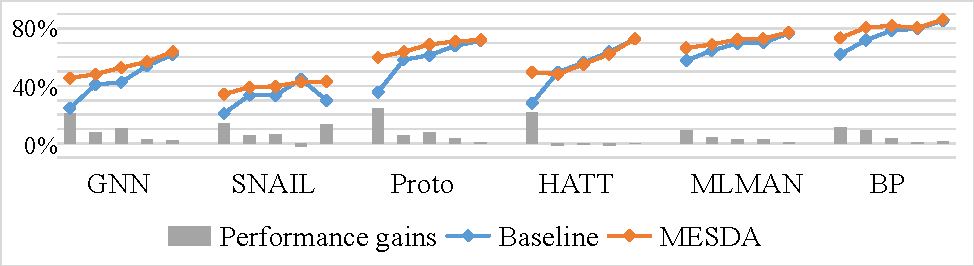
\includegraphics[width=1\linewidth]{51.pdf}
%%\caption{fig1}
%\end{minipage}%
%}%
%\subfigure[5 way 5 shot]{
%\begin{minipage}[t]{0.49\linewidth}
%\centering
%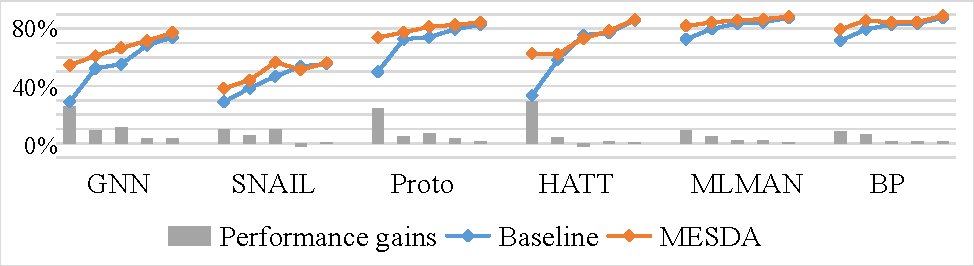
\includegraphics[width=1\linewidth]{55.pdf}
%%\caption{fig2}
%\end{minipage}%
%} \\%
%\subfigure[10 way 1 shot]{
%\begin{minipage}[t]{0.49\linewidth}
%\centering
%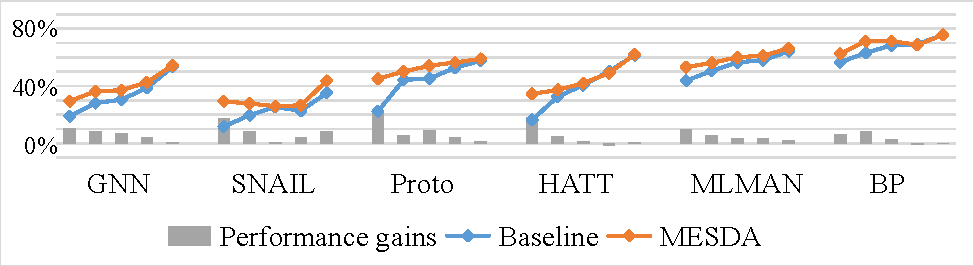
\includegraphics[width=1\linewidth]{101.pdf}
%%\caption{fig2}
%\end{minipage}
%}%
%\subfigure[10 way 5 shot]{
%\begin{minipage}[t]{0.49\linewidth}
%\centering
%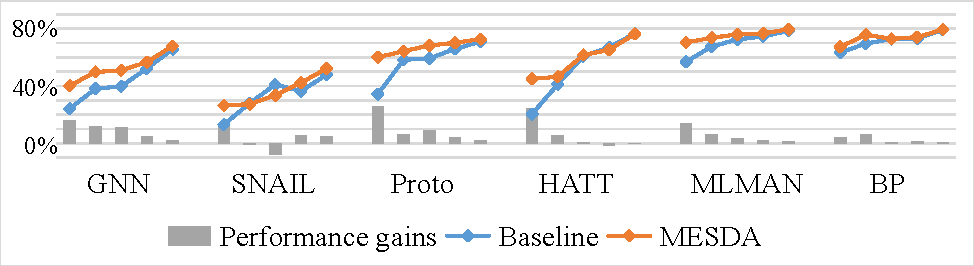
\includegraphics[width=1\linewidth]{105.pdf}
%%\caption{fig2}
%\end{minipage}
%}%
%
%\centering
%\caption{Classification accuracy on FewRel validation set with training data shrunken under N way K shot configurations. Training data is shrunken to 0.22\%, 1.00\%, 2.23\%, 7.00\%, and 100.00\% of full training set size, respectively. For each shrunken training set, we apply baseline models and models with MESDA framework.}
%\label{fig:analysis}
%\end{figure*}

\begin{figure*}[htp]
\centering
\small
\subfigure[5 way 1 shot]{
\centering
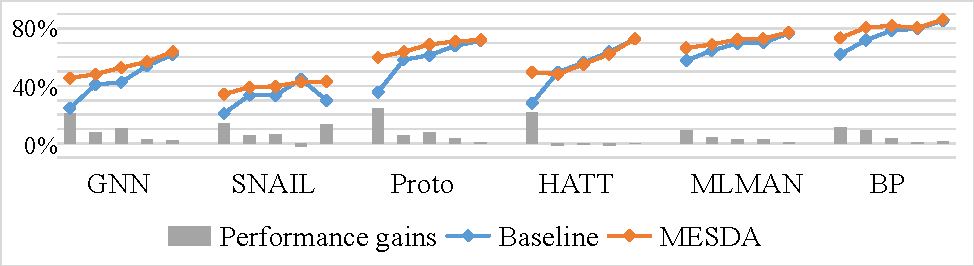
\includegraphics[width=0.49\linewidth]{51.pdf}
%\caption{fig1}
}%
\subfigure[5 way 5 shot]{
\centering
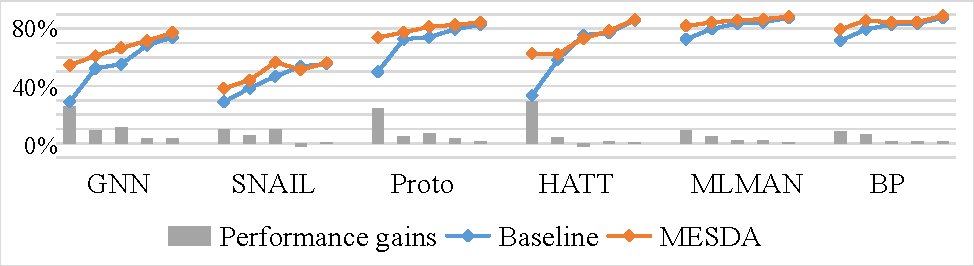
\includegraphics[width=0.49\linewidth]{55.pdf}
%\caption{fig2}
} \\%
\subfigure[10 way 1 shot]{
\centering
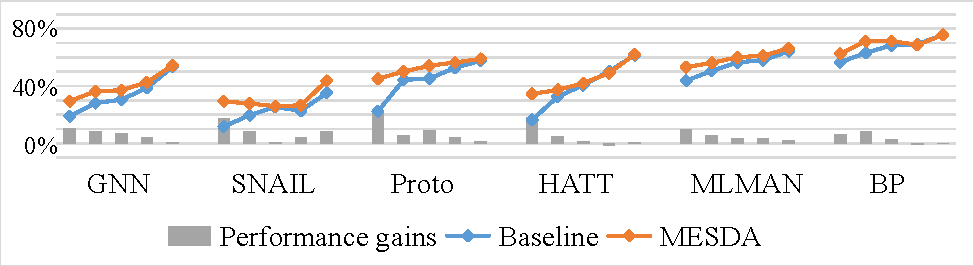
\includegraphics[width=0.49\linewidth]{101.pdf}
%\caption{fig2}
}%
\subfigure[10 way 5 shot]{
\centering
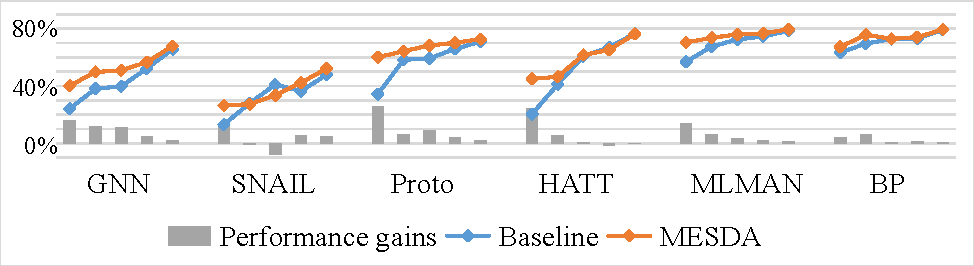
\includegraphics[width=0.49\linewidth]{105.pdf}
%\caption{fig2}
}%

\centering
\caption{Classification accuracy on FewRel validation set with training data shrunken under $N$ way $K$ shot configurations. For each group, from the left to the right, training data is shrunken to 0.22\%, 1.00\%, 2.23\%, 7.00\%, and 100.00\% of full training set size, respectively. For each shrunken training set, we apply baseline models and models with MESDA framework. }
%Proto, HATT, MA, and BP stand for Prototypical Networks, Proto-HATT, MLMAN, and Bert-Pair, respectively.}
\label{fig:analysis}
\end{figure*}

\footnotetext[3]{Using code provided by Ye and Ling \shortcite{ye-ling-2019-multi} with same parameters. Their reported results were 79.01, 88.86, 67.37, and 80.07.}


\subsubsection{Ablation tests}

Here, we focus on the individual effects of support classifier and data augmentation on baseline models. %We facilitate baseline models with either MSI framework or data augmentation and compare the performance with both baseline models and models with

As is shown in Table \ref{FewRelvalAll} and Table \ref{FRMresult}, in most cases, either adding support classifier or data augmentation improves performance for baseline models.
%and either removing support classifier or data augmentation leads to performance decrease from the models trained with both methods.
This illustrates that both support classifier and data augmentation contribute to better performance.

On FewRel dataset (Table \ref{FewRelvalAll}), the support classifier brings more performance gains for poor baselines such as GNN and SNAIL than strong ones such as MLMAN and Bert-Pair. This is because the support classifier makes up for the insufficient learning ability for poor models while is icing on the cake for strong models with sufficient training data.
Improvement of data augmentation is stable on strong baselines while fluctuates on poor ones. This reflects the unstableness of poor baselines. With defects in learning ability, supplementary data brings harder tasks and may confuse poor models, and this is why sometimes data augmentation brings negative gains.
The improvement is more obvious on TinyRel-CM dataset with either support classifier or data augmentation.
%On FewRel dataset (Table \ref{FewRelvalAll}), for strong baselines like MLMAN and Bert-Pair, data augmentation brings more improvement than support classifier, because these models are capable of learning
%extra information
%from cross-domain corpus.
%However, for poor baselines like GNN and SNAIL, support classifier is more powerful
%%than data augmentation
%, because these models do not fully digest information within original training data. Support classifier helps these baselines to learn better while data augmentation brings harder problems and may confuse these models, and this is why sometimes data augmentation brings negative gains.
%This problem does not appear on TinyRel-CM dataset (Table \ref{FRMresult}) because of the small training data size.

\subsubsection{FewRel dataset with reduced training data}
%Table \ref{FewRelval} shows the experimental results on the FewRel dataset. We either keep the original training set or shrink the training set to different extents and test on the validation set. Table \ref{FewRelval} illustrates the strength of our framework and data augmentation method since performance gains are attained in most cases. While the MSI framework keeps helping models to leaner better, data augmentation tends to be more effective when training data is quite limited.
%Figure \ref{fig:analysis} shows the performance gains on MLMAN using MSI framework and data augmentation. The less the training data, the more improvement the model gains, indicating that the MSI framework and data augmentation method's effectiveness under extremely limited training data.

Figure \ref{fig:analysis} shows the performance comparison between baseline models and our methods given different amount of training data on FewRel dataset. As is shown, performance of models deteriorates with the decrease of training data size. For example, the prototypical networks achieves 58.58\% accuracy with full training data under 10 way 1 shot test tasks, but performs poorly with less than 30\% accuracy given only 0.22\% of full training data.

Our framework fits situations where only limited training data is available. As is shown in Figure \ref{fig:analysis}, with our methods, the less the training data, the more improvement the model tends to gain. This indicates the effectiveness of our framework under extremely limited training data. While our methods only improve prototypical networks by 1.27\% accuracy with full training data under 10 way 1 shot test tasks, it leads to about 20\% improvement given 0.22\% of full training data.

%
%\begin{figure}[ht]
%    \centering
%    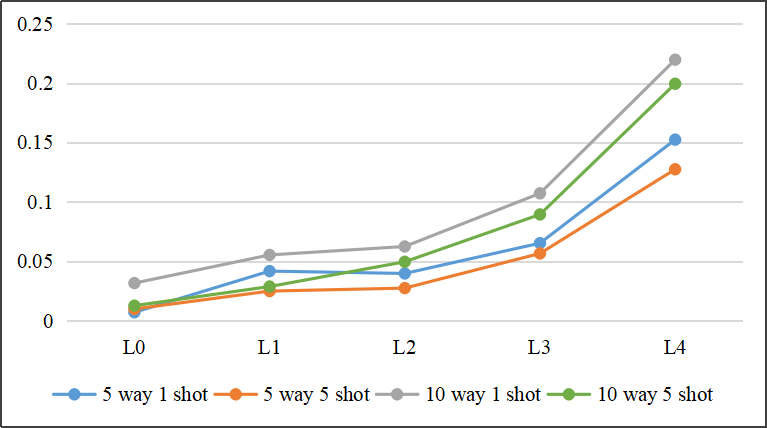
\includegraphics[width=8cm]{analysis.png}
%    \caption{Performance gains(\%) on MLMAN with MSI framework and data augmentation over different scales of training data.}
%    \label{fig:analysis}
%\end{figure}


%Our proposed MME framework outperform all the baselines. We claim that our MME framework is especially suitable for solving \emph{hard tasks}.
%The test group \emph{DISEASE-DISEASE} is \emph{hard} because the test relations in this group are quite different from others. Group \emph{SYMPTOM-FOOD} is relatively easier because other groups like \emph{DISEASE-FOOD} contains similar relations. For easier tasks, only extracting lexical shallow knowledge may contribute to a good performance. But for hard tasks, only digging deep underlying knowledge can a model achieve good results. Experimental results show our proposed MME framework helps with digging deep information of training data.
